\documentclass[11pt]{article}
\usepackage{fullpage}
\usepackage{amsmath,amsthm,amssymb,amsfonts,multirow}
\usepackage{mathtools}
\usepackage{graphicx}
\usepackage{xcolor}
\usepackage{float}
%\usepackage{enumerate}
\usepackage[shortlabels, inline]{enumitem}
\usepackage{textcomp}
\usepackage{hyperref}
\usepackage{comment}

\usepackage{listings}
\lstset{language=Python, numbers=left, basicstyle=\ttfamily, keywordstyle=\color{blue}, showstringspaces=false}

\usepackage[style=alphabetic-verb]{biblatex}
% \bibliography{Problems/ref.bib}

\newcommand{\N}{\mathbb{N}}
\newcommand{\Z}{\mathbb{Z}}
\newcommand{\Q}{\mathbb{Q}}
\newcommand{\R}{\mathbb{R}}
\newcommand{\C}{\mathcal{C}}
\newcommand{\K}{\mathbb{K}}
\renewcommand{\div}{\mid}
\newcommand{\ndiv}{\nmid}
\newcommand{\E}{\mathbb{E}}
\newcommand{\I}{\mathbb{I}}
\newcommand{\F}{\mathcal{F}}

\DeclareMathOperator{\id}{Id}
\DeclareMathOperator{\tr}{Tr}
\DeclareMathOperator*{\argmax}{arg\,max}
\DeclareMathOperator{\lcm}{lcm}
\DeclareMathOperator{\spn}{span}
\DeclareMathOperator{\acosh}{acosh}

\DeclarePairedDelimiter{\floor}{\lfloor}{\rfloor}
\DeclarePairedDelimiter{\ceil}{\lceil}{\rceil}
\DeclarePairedDelimiter{\abs}{\lvert}{\rvert}

\newcommand{\subtag}[1]{\tag{\theparentequation#1}}

\renewcommand{\vec}[1]{\mathbf{#1}}

\usepackage{subfiles}
\usepackage{subcaption}
\makeatletter
\newcommand\nocaption{
    \renewcommand\p@subfigure{}
    \renewcommand{\thesubfigure}{\arabic{figure}\alph{subfigure}}
}
\makeatother


\newenvironment{problem}[2][Question]{\begin{trivlist}
\item[\hskip \labelsep {\bfseries #1}\hskip \labelsep {\bfseries #2.}]}{\end{trivlist}}

\newenvironment{solution}{%
  \begin{proof}[\textbf{Solution}]$ $\par\nobreak\ignorespaces
}{%
  \end{proof}
}

\theoremstyle{definition}
\newtheorem{definition}{Definition}
\newtheorem{theorem}{Theorem}
\newtheorem{lemma}{Lemma}

\hypersetup{
    colorlinks=true,
    linkcolor=blue,
    filecolor=magenta,      
    urlcolor=cyan,
    pdftitle={Overleaf Example},
    pdfpagemode=FullScreen,
    }

%\parskip .125in

\begin{document}
\begin{center}
{\bf Intro to Computational Math, Fall 2025\\
Homework 7 Sample Solutions}
\end{center}

{\bf Question 1.}
Here we have
\[
f(x)=\ln(x), \qquad f''(x)=-\frac{1}{x^{2}}.
\]
On \([1,2]\), \(\max_{t\in[1,2]}\lvert f''(t)\rvert=1\). Hence the piecewise linear interpolation error bound from lecture implies
\[
\max_{x\in[1,2]}\lvert \ln(x)-p(x)\rvert \le 1\cdot h^{2} = 10^{-4}.
\]
Since \(f''(x)<0\) on \([1,2]\), \(f\) is concave, so \(p(x)\le f(x)\) and the largest error occurs near midpoints of subintervals where \(\lvert f''\rvert\) is largest, i.e., close to \(x=1\).

% Code (verbatim) and numerical report
\noindent\textbf{Code and numerical results.} The following Python produces the plot of \(f(x)-p(x)\), reports the maximum error, and overlays the theoretical bound.

\begin{lstlisting}
import numpy as np
import matplotlib.pyplot as plt

# nodes and function values
x_nodes = np.linspace(1.0, 2.0, 101)           # 1.00, 1.01, ..., 2.00
y_nodes = np.log(x_nodes)

# fine grid for plotting the error
x = np.linspace(1.0, 2.0, 200_001)
y = np.log(x)
y_lin = np.interp(x, x_nodes, y_nodes)         # piecewise linear interpolant
err = y - y_lin

# theoretical uniform bound
h = 0.01
bound = h**2

# report the maximum absolute error and where it occurs
imax = np.argmax(np.abs(err))
print("max |err| =", float(np.abs(err[imax])))
print("argmax x   =", float(x[imax]))
print("theoretical bound =", float(bound))

# plot f(x) - p(x)
plt.figure(figsize=(6,3.6))
plt.plot(x, err, linewidth=1.2)
plt.axhline(+bound, linestyle="--")
plt.axhline(-bound, linestyle="--")
plt.xlabel("x")
plt.ylabel("ln(x) - linear interpolant")
plt.title("Piecewise linear interpolation error for ln on [1,2] with h=0.01")
plt.tight_layout()
plt.savefig("Q1_log_interp_error.pdf", dpi=200)
plt.show()
\end{lstlisting}

\begin{center}
    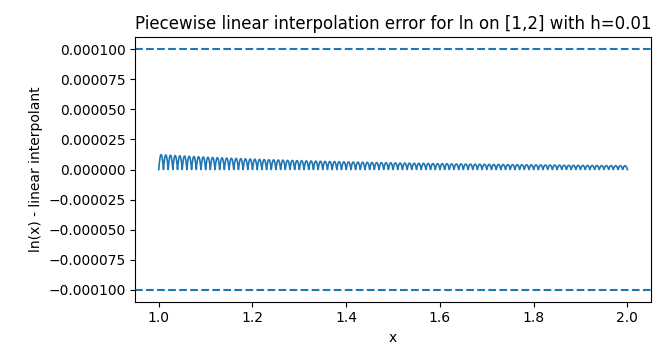
\includegraphics[width=0.8\textwidth]{hw7_1_fig.png}
\end{center}
A representative run yields
\[
\max_{x\in[1,2]}\lvert \ln(x)-p(x)\rvert \approx 1.2376117048\times 10^{-5} \text{ at } x\approx 1.00499,
\]
which is below the bound \(10^{-4}\) and occurs near the midpoint of the first subinterval. With a stronger result than we proved in class, a bound eight times stronger of $1.25\times 10^{-5}$ could be proven, which closely matches this observed error.


\newpage



{\bf Question 2.}
Let \(f\) be \(C^{2}\) on \([a,b]\) and let \(h=(b-a)/n\). For piecewise linear interpolation \(p_{1}\) on a uniform grid,
\[
\lVert f-p_{1}\rVert_{\infty}\le \lVert f''\rVert_{\infty}h^{2}.
\]
If \(f\in C^{4}\) and \(s\) is the natural cubic spline interpolant,
\[
\lVert f-s\rVert_{\infty}\le C\lVert f^{(4)}\rVert_{\infty}h^{4},
\]
for a constant \(C\) independent of \(h\). Thus, on a loglog plot of error versus \(n\), the observed slopes should be approximately \(-2\) and \(-4\), respectively.

We measure errors in the infinity norm on a fine grid for each case
\[
\text{(a)}\quad f(x)=\cos(\pi x^{2}) \text{ on } [0,4],\qquad
\text{(b)}\quad f(x)=\ln(x) \text{ on } [1,20],\qquad
\text{(c)}\quad f(x)=\sin(1/x) \text{ on } [1/2,7].
\]

\begin{lstlisting}
import numpy as np
import matplotlib.pyplot as plt

# ---------- cubic spline with NOT-A-KNOT boundary conditions ----------

def not_a_knot_spline(x, y):
    """
    Return an evaluator for the cubic spline through (x,y) with not-a-knot BCs.
    Works for nonuniform x as well. No SciPy used.
    """
    x = np.asarray(x, dtype=float)
    y = np.asarray(y, dtype=float)
    n = len(x) - 1
    h = np.diff(x)                         # h[i] = x[i+1] - x[i]

    # Unknowns: second derivatives m[0..n]
    A = np.zeros((n+1, n+1))
    rhs = np.zeros(n+1)

    # Interior equations: i = 1..n-1
    for i in range(1, n):
        A[i, i-1] = h[i-1]
        A[i, i]   = 2*(h[i-1] + h[i])
        A[i, i+1] = h[i]
        rhs[i] = 6*((y[i+1]-y[i])/h[i] - (y[i]-y[i-1])/h[i-1])

    # Not-a-knot at x1: (m1 - m0)/h0 = (m2 - m1)/h1
    A[0, 0] = -1.0/h[0]
    A[0, 1] =  1.0/h[0] + 1.0/h[1]
    A[0, 2] = -1.0/h[1]
    rhs[0] = 0.0

    # Not-a-knot at x_{n-1}: (mn - m_{n-1})/h_{n-1} = (m_{n-1} - m_{n-2})/h_{n-2}
    A[n, n]     =  1.0/h[n-1]
    A[n, n-1]   = -1.0/h[n-1] - 1.0/h[n-2]
    A[n, n-2]   =  1.0/h[n-2]
    rhs[n] = 0.0

    m = np.linalg.solve(A, rhs)

    def eval_spline(xq):
        xq = np.asarray(xq, dtype=float)
        i = np.searchsorted(x, xq, side='right') - 1
        i = np.clip(i, 0, n-1)
        xi, xi1 = x[i], x[i+1]
        hi = xi1 - xi
        # second-derivative (M) form
        term1 = m[i]*(xi1 - xq)**3/(6*hi)
        term2 = m[i+1]*(xq - xi)**3/(6*hi)
        term3 = (y[i] - m[i]*hi*hi/6.0)*(xi1 - xq)/hi
        term4 = (y[i+1] - m[i+1]*hi*hi/6.0)*(xq - xi)/hi
        return term1 + term2 + term3 + term4

    return eval_spline

# ---------- utilities shared by all cases ----------

def piecewise_linear(xnodes, ynodes, xq):
    return np.interp(xq, xnodes, ynodes)

def run_case(f, a, b, n_values, name, fine_points=1600):
    xfine = np.linspace(a, b, fine_points)
    yfine = f(xfine)
    errs_lin, errs_cub = [], []

    for n in n_values:
        xnodes = np.linspace(a, b, n+1)
        ynodes = f(xnodes)

        ylin = piecewise_linear(xnodes, ynodes, xfine)
        errs_lin.append(np.max(np.abs(yfine - ylin)))

        S = not_a_knot_spline(xnodes, ynodes)
        ys = S(xfine)
        errs_cub.append(np.max(np.abs(yfine - ys)))

    errs_lin = np.array(errs_lin)
    errs_cub = np.array(errs_cub)
    nvals = np.array(n_values, dtype=float)

    # empirical loglog slopes on the last few points
    k = min(4, len(nvals))
    slope_lin = np.polyfit(np.log(nvals[-k:]), np.log(errs_lin[-k:]), 1)[0]
    slope_cub = np.polyfit(np.log(nvals[-k:]), np.log(errs_cub[-k:]), 1)[0]
    print(f"{name}: slope linear ~ {slope_lin:.3f}  slope cubic ~ {slope_cub:.3f}")

    # reference lines normalized at the last point
    ref2 = errs_lin[-1]*(nvals/nvals[-1])**(-2)
    ref4 = errs_cub[-1]*(nvals/nvals[-1])**(-4)

    plt.figure(figsize=(6,3.6))
    plt.loglog(nvals, errs_lin, 'o-', label='piecewise linear')
    plt.loglog(nvals, errs_cub, 's-', label='cubic spline (not-a-knot)')
    plt.loglog(nvals, ref2, '--', label='n^{-2} reference')
    plt.loglog(nvals, ref4, '--', label='n^{-4} reference')
    plt.xlabel("n")
    plt.ylabel("max error on a fine grid")
    plt.title(name + "  error vs n (loglog)")
    plt.legend()
    plt.tight_layout()
    plt.show()

# ---------- run the three textbook cases ----------

# (a) cos(pi x^2) on [0,4]
f_a = lambda x: np.cos(np.pi * x * x)
n_values_a = [10,20,40,80,160,320,640]
run_case(f_a, 0.0, 4.0, n_values_a, name="cos(pi x^2) on [0,4]")

# (b) ln(x) on [1,20]
f_b = lambda x: np.log(x)
n_values_b = [10,20,40,80,160,320,640]
run_case(f_b, 1.0, 20.0, n_values_b, name="ln(x) on [1,20]")

# (c) sin(1/x) on [1/2,7]
f_c = lambda x: np.sin(1.0/x)
n_values_c = [10,20,40,80,160,320,640]
run_case(f_c, 0.5, 7.0, n_values_c, name="sin(1/x) on [1/2,7]")
\end{lstlisting}
\begin{center}
    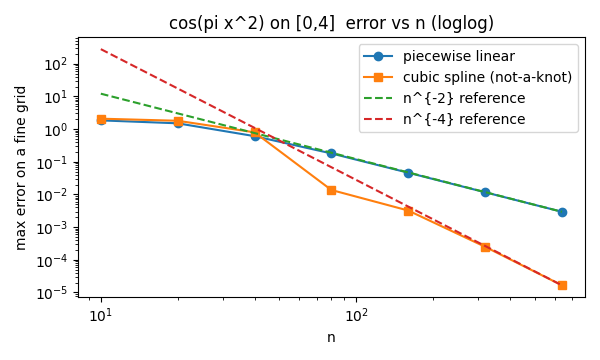
\includegraphics[width=0.7\textwidth]{hw7_2_fig1.png}
    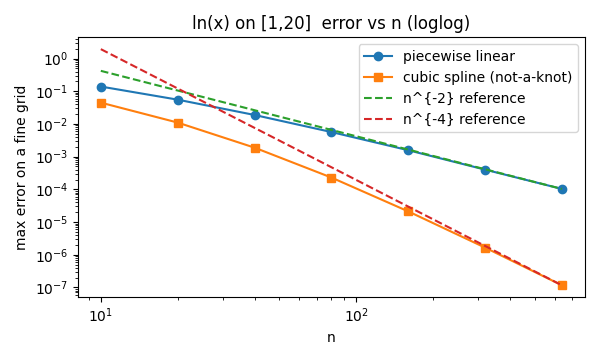
\includegraphics[width=0.7\textwidth]{hw7_2_fig2.png}
    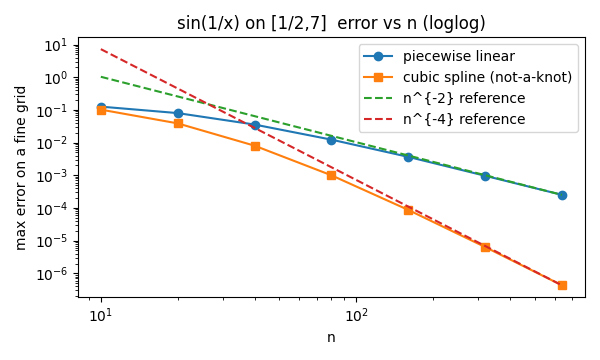
\includegraphics[width=0.7\textwidth]{hw7_2_fig3.png}
\end{center}


\newpage



{\bf Question 3.}

\noindent\emph{(i) Piecewise linear interpolation.}
For \(t\in[t_{k-1},t_{k}]\),
\[
S_{k}(t)=\begin{bmatrix} a_{k}+b_{k}\tau \\ d_{k}+e_{k}\tau \end{bmatrix},\qquad \tau=t-t_{k-1}.
\]
Imposing \(S_{k}(t_{k-1})=[x_{k-1}\;y_{k-1}]^{T}\) and \(S_{k}(t_{k})=[x_{k}\;y_{k}]^{T}\) yields
\[
a_{k}=x_{k-1},\quad b_{k}=x_{k}-x_{k-1},\qquad d_{k}=y_{k-1},\quad e_{k}=y_{k}-y_{k-1},
\]
so
\[
S_{k}(t)=\begin{bmatrix} x_{k-1}+(x_{k}-x_{k-1})\tau \\ y_{k-1}+(y_{k}-y_{k-1})\tau \end{bmatrix},\qquad \tau\in[0,1].
\]

\noindent\emph{(ii) Quadratic \(C^{1}\) interpolation.}
For \(t\in[t_{k-1},t_{k}]\),
\[
S_{k}(t)=\begin{bmatrix} a_{k}+b_{k}\tau+c_{k}\tau^{2} \\ d_{k}+e_{k}\tau+f_{k}\tau^{2} \end{bmatrix},\qquad \tau=t-t_{k-1}.
\]
Value interpolation at the endpoints gives \(a_{k}=x_{k-1}\) and \(b_{k}+c_{k}=x_{k}-x_{k-1}\). Derivatives are \(S_{k}'(t)=[b_{k}+2c_{k}\tau\;\; e_{k}+2f_{k}\tau]^{T}\). Enforcing \(C^{1}\) continuity at interior nodes \(t_{k}\) gives
\[
b_{k+1}=b_{k}+2c_{k},\qquad e_{k+1}=e_{k}+2f_{k},\qquad k=1,\dots,7.
\]
To close the system, we could, for exampl,e impose that
\[
b_{1}=x_{1}-x_{0},\qquad e_{1}=y_{1}-y_{0}.
\]
These equations determine \((b_{k},c_{k})\) and \((e_{k},f_{k})\) uniquely. On each segment,
\[
\begin{bmatrix} x(t) \\ y(t) \end{bmatrix}=
\begin{bmatrix} x_{k-1}+b_{k}\tau+c_{k}\tau^{2} \\ y_{k-1}+e_{k}\tau+f_{k}\tau^{2} \end{bmatrix},\qquad \tau\in[0,1].
\]

\noindent\textbf{Python code.} The script builds both interpolants with the \(\tau=t-t_{k-1}\) convention and plots the resulting trajectories.

\begin{lstlisting}
import numpy as np
import matplotlib.pyplot as plt

# Data and times
xk = np.array([0,1,2,3,2,1,0,0,0], dtype=float)
yk = np.array([0,3,3,4,5,4,6,8,10], dtype=float)
tk = np.arange(len(xk), dtype=float)  # 0..8
nseg = len(xk) - 1  # 8

# ---------- (i) piecewise linear with tau = t - t_{k-1} ----------
def eval_linear(t):
    t = np.atleast_1d(t)
    k = np.floor(t).astype(int) + 1            # 1..nseg
    k = np.clip(k, 1, nseg)
    tau = t - (k - 1)                           # in [0,1]
    xl = xk[k-1] + (xk[k] - xk[k-1]) * tau
    yl = yk[k-1] + (yk[k] - yk[k-1]) * tau
    return xl, yl

# ---------- (ii) quadratic C1 with tau = t - t_{k-1} ----------
def solve_quadratic_C1(vals):
    # Unknowns: u = [b1,c1,b2,c2,...,b_nseg,c_nseg]
    m = 2 * nseg
    A = np.zeros((m, m))
    rhs = np.zeros(m)
    r = 0

    # Endpoint values: b_k + c_k = vals[k] - vals[k-1]
    for k in range(1, nseg+1):
        ib = 2*(k-1); ic = ib+1
        A[r, ib] = 1.0
        A[r, ic] = 1.0
        rhs[r] = vals[k] - vals[k-1]
        r += 1

    # C1 continuity at interior nodes: b_{k+1} - b_k - 2 c_k = 0
    for k in range(1, nseg):
        ibk = 2*(k-1)
        ibkp1 = 2*k
        ick = 2*(k-1) + 1
        A[r, ibkp1] = 1.0
        A[r, ibk]   = -1.0
        A[r, ick]   = -2.0
        rhs[r] = 0.0
        r += 1

    # Clamped at t0: b1 = forward difference
    A[r, 0] = 1.0
    rhs[r] = vals[1] - vals[0]
    r += 1
    assert r == m

    u = np.linalg.solve(A, rhs)
    b = u[0::2]
    c = u[1::2]
    return b, c

bx, cx = solve_quadratic_C1(xk)
by, cy = solve_quadratic_C1(yk)

def eval_quadratic(t):
    t = np.atleast_1d(t)
    k = np.floor(t).astype(int) + 1
    k = np.clip(k, 1, nseg)
    tau = t - (k - 1)
    xq = xk[k-1] + bx[k-1]*tau + cx[k-1]*(tau**2)
    yq = yk[k-1] + by[k-1]*tau + cy[k-1]*(tau**2)
    return xq, yq

# Sanity checks: interpolation and C1 continuity
tt_nodes = tk
xq_nodes, yq_nodes = eval_quadratic(tt_nodes)
assert np.allclose(xq_nodes, xk) and np.allclose(yq_nodes, yk)
for k in range(1, nseg):
    left_dx = bx[k-1] + 2*cx[k-1]              # S_k'(t_k)
    right_dx = bx[k]                           # S_{k+1}'(t_k)
    left_dy = by[k-1] + 2*cy[k-1]
    right_dy = by[k]
    assert np.allclose([left_dx, left_dy], [right_dx, right_dy])

# ---------- plotting ----------
tt = np.linspace(0.0, 8.0, 4001)
xL, yL = eval_linear(tt)
xQ, yQ = eval_quadratic(tt)

plt.figure(figsize=(5.6,5.2))
plt.plot(xL, yL, '-', label='piecewise linear')
plt.plot(xQ, yQ, '-', label='quadratic C1')
plt.plot(xk, yk, 'o', label='data points')
plt.axis('equal')
plt.xlabel("x(t)")
plt.ylabel("y(t)")
plt.title("Interpolated whale trajectory (tau = t - t_{k-1})")
plt.legend()
plt.tight_layout()
plt.savefig("Q3_interpolated_paths_tau_left.pdf", dpi=200)
plt.show()
\end{lstlisting}
\begin{center}
    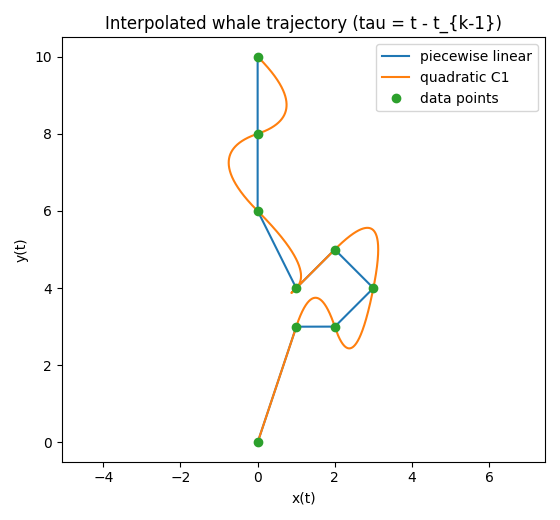
\includegraphics[width=0.8\textwidth]{hw7_3_fig.png}
\end{center}




\end{document}
